\section{Implementation Details}
\subsection{DLO Representation}
\label{sec:DLORepr}

In this work, we mainly follow discrete elastic rod~\citep{bergou2008discrete,bergou2010discrete} methods to model deformable linear objects (DLOs).
Concretely, a DLO $\rmX$ is a centerline given by a set of $\text{N}_v$ vertices $\{\rvx_i\}_{i=1}^{\text{N}_v}$ and a set of $\text{N}_e$ orthonormal material frames $\{(\rvd_1, \rvd_2, \rvd_3)^j\}_{j=1}^{\text{N}_e}$ attached to each edge $\rve^j=\rvx_{j+1}-\rvx_j$. Each vertex has its mass $m_i$ and radius $r_i$. Note that we use lower and upper indices to specify vertex- and edge-based properties, respectively.
We assume $\rvd_3^j$ is adapted to the tangent $\rvt^j$ to the centerline, \ie, $\rvd_3^j \equiv \rvt^j = \rve^j/|\rve^j|$.  At the initial time $t=0$, we predefine a reference frame $(\underline{\rvd}_1, \underline{\rvd}_2, \underline{\rvd}_3)$. The material frame can be obtained at a later time through a twist angle $\theta^j$ with respect to the reference frame. Thus, the total degrees of freedom (DoF) associated with the DLO, given by $\text{N}_v$ vertices and $\text{N}_e$ twist angles, is $3\times \text{N}_v+\text{N}_e$.

To achieve elastic simulation for a DLO, we need to compute its elastic potential as defined by strain. Based on Kirchhoff’s rod model~\citep{dill1992kirchhoff,o2017kirchhoff}, strains can be separated into three categories: stretching, bending, and twisting.
\begin{itemize}[leftmargin=10pt]
    \item \textbf{Stretching} The stretching strain, or axial strain of an edge $\rve^j$ is given by:
    \begin{equation}
        \epsilon^j=\frac{|\rve^j|}{|\bar{\rve}^j|}-1,
    \end{equation}
    where $|\bar{\rve}^j|$ is the rest edge length. Denote $k_s^j=KA^j$ as the stretching stiffness, where $K$ is the stretching modulus and $A^j$ is the cross-sectional area, the stretching energy is then defined as:
    \begin{equation}
        U_s=\frac{1}{2}\sum_{j=1}^{\text{N}_e} k_s^j \big(\epsilon^j\big)^2\big|\bar{\rve}^j\big|.
    \end{equation}
    \item \textbf{Bending} The bending strain for an internal vertex $\rvx_i$ is defined by the curvature binormal $(\kappa\rvb)_i$, which captures the misalignment between two adjacent edges:
    \begin{equation}
        (\kappa\rvb)_i=\frac{2\rvt^{i-1}\times \rvt^i}{1+\rvt^{i-1}\cdot \rvt^i}.
    \end{equation}
    Note that $|(\kappa\rvb)_i| = 2\tan(\phi_i/2)$, where $\phi_i$ is the bending angle between consecutive edges. The material curvature at an interior vertex is defined as
    \begin{equation}
        \boldsymbol{\kappa}_i=\frac{1}{2}\sum_{j=i-1}^i\left((\kappa \rvb)_i\cdot \rvd_2^j, (\kappa \rvb)_i\cdot \rvd_1^j\right)^\top.
    \end{equation}
    With these properties defined, we can formulate the bending energy as:
    \begin{equation}
        U_b = \frac{1}{2}\sum_{i=2}^{\text{N}_v-1}\frac{1}{\bar{l}_i}(\boldsymbol{\kappa}_i-\bar{\boldsymbol{\kappa}}_i)^\top B_i (\boldsymbol{\kappa}_i-\bar{\boldsymbol{\kappa}}_i),
    \end{equation}
    where $\bar{l}_i=(|\bar{\rve}^{i-1}|+|\bar{\rve}^{i}|)/2$ is the Voronoi length for a vertex, $\boldsymbol{\bar{\kappa}}_i$ is the undeformed curvature,
    \begin{equation}
        B_i=\frac{EA_i}{4}
        \begin{pmatrix}
            r_i^2 & 0 \\
            0 & r_i^2
        \end{pmatrix},
    \end{equation}
    is the bending stiffness, $E$ is the bending modulus.
    \item \textbf{Twisting} The twisting strain is defined as:
    \begin{equation}
        \tau_i = m_i-\bar{m}_i,
    \end{equation}
    where $m_i=\theta^i-\theta^{i-1}+\underline{m}_i$, $\bar{m}_i$ is the undeformed twist, and $\underline{m}_i$ is the reference twist. Given the twisting stiffness $\beta_i=GA_i r_i^2/2$, where $G$ is the twisting modulus, the twisting energy writes as:
    \begin{equation}
        U_t=\frac{1}{2}\sum_{i=2}^{\text{N}_v-1}\beta_i\frac{\big(\tau_i\big)^2}{\bar{l}_i}.
    \end{equation}
\end{itemize}

\paragraph{Inextensibility Constraint} In addition, when inextensibility is desired, we can deactivate the stretching energy and use the following geometry projections to enforce the constraint. This approach directly modifies vertex positions to satisfy length constraints, offering greater stability than high-stiffness penalty forces. For each edge $\rve^j$ connecting vertices $\rvx_j$ and $\rvx_{j+1}$, we first evaluate the constraint function $C(\rvx_j, \rvx_{j+1}) = |\rvx_{j+1} - \rvx_j| - |\bar{\rve}^j|$, where $|\bar{\rve}^j|$ is the rest edge length. A correction vector $\Delta \rvx$ is then calculated for each vertex, weighted by its inverse mass $w_i = 1/m_i$. The correction is distributed along the tangent vector $\rvt^j$, as shown in the following equations: 
\begin{equation}
\begin{split}
    \lambda &= \frac{C(\rvx_j, \rvx_{j+1})}{w_j + w_{j+1}},\\
    \Delta \rvx_j &= \lambda w_j \cdot \rvt^j,\\
    \Delta \rvx_{j+1} &= -\lambda w_{j+1} \cdot \rvt^j.
\end{split}
\end{equation}
 Finally, the vertex positions are updated via $\rvx_j = \rvx_j + \Delta \rvx_j$ and $\rvx_{j+1} = \rvx_{j+1} + \Delta \rvx_{j+1}$. This process is repeated for $N_C$ iterations to enforce the inextensibility of the DLO robustly.

 \paragraph{Bending Plasticity}
 To simulate elastoplastic materials such as metal wires that can be permanently deformed, we keep track of the rest curvature $\bar{\boldsymbol{\kappa}}_i$ for each internal vertex $i$. 
Plastic deformation occurs when the magnitude of the elastic curvature $\boldsymbol{\kappa}^{el}_i=\boldsymbol{\kappa}_i - \bar{\boldsymbol{\kappa}}_i$ exceeds a predefined yield threshold, $\sigma_y$. If $|\boldsymbol{\kappa}_i^{el}| > \sigma_y$, the rest curvature is updated according to a creep model, which drives the rest curvature towards the current curvature at a rate proportional to the excess strain. The change in rest curvature, $\Delta\bar{\boldsymbol{\kappa}}_i$, for a given timestep is calculated as: 
\begin{equation} 
\Delta\bar{\boldsymbol{\kappa}}_i = r_c \cdot \frac{|\boldsymbol{\kappa}_i^{el}| - \sigma_y}{|\boldsymbol{\kappa}_i^{el}|} \boldsymbol{\kappa}_i^{el},
\end{equation} 
where $r_c$ is the plastic creep rate. This update is then integrated over time, $\bar{\boldsymbol{\kappa}}_i =\bar{\boldsymbol{\kappa}}_i + \Delta\bar{\boldsymbol{\kappa}}_i$, allowing the rod to retain a new intrinsic shape after significant bending.

\paragraph{Loop Topology}
To properly initialize the material frames for a DLO with a closed-loop topology, we must account for the geometric phase, or holonomy, that arises from parallel transport around a non-trivial curve. A naive sequential transport of the material frame from the first edge ($j=1$) to the last ($j=N_e$) results in a discontinuity, as parallel transporting the final frame $\bar{\rvd}_1^{N_e}$ back across the closing edge to the tangent of the first edge, $\rvt^1$, will not align with the original frame $\bar{\rvd}_1^1$. To resolve this, we first compute the total holonomy angle, $\psi_H$, which represents this angular mismatch. We then distribute this error evenly across all edges. For each edge $j$, we compute a local correction angle $\phi^j = - \psi_H \cdot (j-1) / N_e$. The initial, uncorrected material frame vectors, denoted as $\hat{\rvd}_1^j$ and $\hat{\rvd}_2^j$, are then rotated by $\phi^j$ to obtain the final, continuous reference frames for the closed loop:
\begin{equation} \begin{bmatrix} \bar{\rvd}_1^j \\ \bar{\rvd}_2^j \end{bmatrix} = \begin{bmatrix} \cos \phi^j & \sin \phi^j \\ -\sin \phi^j & \cos \phi^j \end{bmatrix} \begin{bmatrix} \hat{\rvd}_1^j \\ \hat{\rvd}_2^j \end{bmatrix}.
\end{equation}
This procedure ensures that the material frame is consistent and continuous across the entire loop at its rest state.

\paragraph{Self-collision and Friction} To handle collisions and frictional contact among DLOs, we employ a hybrid PBD approach that combines geometric projections for non-penetration with velocity-level updates for friction. We model each segment as a continuous cylinder with radius $r_i$. For any pair of potentially colliding edges, defined by vertices $(\rvx_i, \rvx_{i+1})$ and $(\rvx_j, \rvx_{j+1})$, we first compute the closest points between the two line segments. These points, $\rvc_a$ and $\rvc_b$, are found using barycentric coordinates $t$ and $u \in [0, 1]$ such that $\rvc_a = (1-t)\rvx_i + t\rvx_{i+1}$ and $\rvc_b = (1-u)\rvx_j + u\rvx_{j+1}$. The non-penetration constraint is enforced if the penetration depth $d = (r_a + r_b) - |\rvc_a - \rvc_b|$ is positive. A correction vector is then applied to the four defining vertices, weighted by their respective inverse masses and barycentric coordinates. The correction for vertex $\rvx_i$, for example, is calculated as: \begin{equation}
\Delta \rvx_i = \frac{d \cdot w_i (1-t)}{w_i(1-t)^2 + w_{i+1}t^2 + w_j(1-u)^2 + w_{j+1}u^2} \cdot \rvn,
\end{equation}
where $\rvn = (\rvc_a - \rvc_b) / |\rvc_a - \rvc_b|$ is the contact normal. We also repeat the geometric projections for $N_C$ iterations. After the positional correction, friction is resolved at the velocity level. We implement a Coulomb friction model where the tangential velocity update $\Delta\rvv_t$ is proportional to the normal impulse magnitude, which is approximated from the penetration depth $d$. This velocity correction is then distributed to the four vertices, similarly weighted by their inverse masses and barycentric coordinates, to provide a stable and physically plausible contact response.


\subsection{Rendering}

We utilize the customized LuisaRender~\citep{zheng2022luisarender} available in Genesis to create photorealistic images of our simulation results. The enhanced photorealism enables our simulation environment to generate perception training data for policy learning in DLO manipulation, paving the way for future applications.

\section{Environmental Setup}

\begin{table}[t]
    \centering
    \setlength{\tabcolsep}{1.6mm}{
    \begin{tabular}{ccccccc}
    \toprule
        \multirow{2}{*}{\bf Tasks} & \multirow{2}{*}{\bf \#Vertices} & \bf Stretching & \bf Bending & \bf Twisting & \multirow{2}{*}{\bf Inextensibility} & \multirow{2}{*}{\bf Plasticity} \\
        & & \bf Modulus &\bf Modulus &\bf Modulus & & \\
    \midrule
        \bf Coiling & 60 & -- & 1e3 & 1e3 & \checkmark & -- \\
        \bf Gathering & 45 & 1e5 & 1e3 & 1e3 & -- & -- \\
        \bf Lifting & 30  & 1e5 & 5e3 & 1e3 & --& --\\
        \multirow{2}{*}{\bf Separation} & 30  & -- & 5e3 & 1e3 & \checkmark & --\\
        & 30 & -- & 5e3 & 1e3 & \checkmark & --\\
        \bf Slingshot & 12  & 8e5 & 1e5 & -- & -- & --\\
        \bf Unknotting & 50  & 1e5 & 1e4 & -- & -- & --\\
        \bf Wiring-post & 30  & -- & 1e4 & 1e3 & \checkmark & --\\
        \bf Wrapping & 50  & 1e5  & 1e4 & -- & --& --\\
        \multirow{3}{*}{\bf Letter Art} & 24  & 1e5 & 1e4 & -- & -- & \checkmark \\
        & 30  & 1e5 & 1e4 & -- & -- & \checkmark  \\
        & 25  & 1e5 & 2e3 & -- & -- & \checkmark \\
        \bf Wiring-ring & 30  & 1e5 & 1e4 & --& -- &-- \\
    \bottomrule
    \end{tabular}
    }
\caption{\textbf{Parameter settings of DLOs used in our simulation benchmark tasks.}}
\label{tab:sim_params}
\end{table}

\subsection{Task Setup}
\label{sec:task_setup}
In all our manipulation tasks, we set the frame time equal to 1e-3 seconds, and each frame is computed using 5 substeps. For the 8 fixed-horizon tasks, we set the number of frames to 2,000, except for the Slingshot task, where we set it to 800. We report the parameter settings for each simulation task in~\Cref{tab:sim_params}. 

\subsection{Reward Design}
\label{sec:reward_design}
Here, we outline the reward design used for our manipulation tasks.

\textbf{Coiling}\quad The reward is defined as the sum of the negative distances from each vertex of the rope to the center of the cone.

\textbf{Gathering}\quad The reward consists of three parts. (a) Object clustering: The negative sum of pairwise distances between the three target objects. (b) Rope-object contact: The negative minimum distance from the rope vertices to each object. (c) Penalty for naïve solution: $-\sum_{k}\sum_o\max (0, \epsilon-d(\rvp^\mathrm{ef}_k, \rvp_o))$, where $\epsilon=0.1$ is the margin, $\rvp^\mathrm{ef}_k$ denotes the $k$-th end-effector position, and $\rvp_o$ denotes the center-of-mass position of the $o$-th target object. This term discourages the agent from directly using end-effectors to push the target objects together.

\textbf{Lifting}\quad We define the reward function as the sum of four components. (a) Elevation: The sum of the vertical positions of the two target rings. (b) Contact: The negative minimum distance between the rope vertices and the center of each ring. (c) Lifting configuration: A positive reward for positioning the engaging rope vertices slightly above the center of each ring, promoting a stable lifting configuration. (d) Penalty for naïve solution: $-\sum_{k}\sum_r\max (0, \epsilon-d(\rvp^\mathrm{ef}_k, \rvp_r))$, where $\epsilon=0.08$ is the margin, $\rvp^\mathrm{ef}_k$ denotes the $k$-th end-effector position, and $\rvp_r$ denotes the center position of the $r$-th ring. This term enforces indirect manipulation via the rope.

\textbf{Separation}\quad We calculate the Chamfer distance between the two ropes and use it as the reward.

\textbf{Slingshot}\quad The reward is defined as the moving distance of the cube projected onto the +$y$-axis (the direction away from the slingshot) after the slingshot is released.

\textbf{Unknotting}\quad We compute a penalty term composed of two parts, and the reward is the negative of the penalty. (a) Topological complexity: We calculate the discrete Average Crossing Number (ACN) by summing the signed crossing contributions of all non-adjacent edge pairs. (b) Self-repulsion: To prevent the rope from intersecting itself or forming tight, physically implausible clusters during manipulation, we add a heavy penalty for any non-adjacent segments that approach within twice the segment interval.

\textbf{Wiring-post}\quad We define the reward as the sum of three components. (a) Shape alignment: We compute the negative Chamfer distance between the rope vertices and the goal-state positions. (b) Midpoint anchoring: We encourage the midpoint of the rope to align with a designated center point on the $xy$-plane, with a 2cm tolerance. (c) Height penalty: A penalty is applied if any part of the rope exceeds the height of the posts.

\textbf{Wrapping}\quad The reward consists of two parts. (a) Topological winding: we compute the discrete Winding Number for the rope relative to each post by summing the signed angles between consecutive rope segments in the $xy$-plane. The reward is maximized when the magnitude of this winding number approaches 1.0 (\ie, one full revolution) for every post. (b) Surface contact: To tighten the loop, we penalize the minimum distance between the rope and each post.

Note that we apply the exponential or translational transformation to the reward function when necessary to ensure it is non-negative. The loss used for gradient-based methods is typically defined by the negative rewards in those tasks.

For \textbf{Letter Art} and \textbf{Wiring-ring}, the reward for each sub-task is obtained from the DLO agent. Please see Appendix~\ref{sec:details_dlo_agent} for detailed prompts.

\begin{table}[h]
    \centering
    \small % Slightly reduce font size to fit 3 tables side-by-side
    
    \begin{minipage}[t]{0.23\textwidth}
        \centering
        \scalebox{0.9}{
        \setlength{\tabcolsep}{1mm}{
        \begin{tabular}{l|c}
            \hline
            actor lr & 5e-4 \\
            actor mlp & [256, 128, 64] \\
            critic lr & 5e-4 \\
            critic mlp & [256, 128, 64] \\
            grad clip & 0.5 \\
            GAE $\lambda$ & 0.95\\
            entropy coeff. & 5e-3 \\
            % \multicolumn{2}{l}{} \\ % Empty row to align bottom lines roughly
            \hline
        \end{tabular}
        }}
        \caption{\bf PPO parameters.}
        \label{tab:ppo_params}
    \end{minipage}
    \hfill
    \begin{minipage}[t]{0.23\textwidth}
        \centering
        \scalebox{0.9}{
        \setlength{\tabcolsep}{1mm}{
        \begin{tabular}{l|c}
            \hline
            actor lr & 5e-4 \\
            actor mlp & [256, 128, 64] \\
            critic lr & 5e-4 \\
            critic mlp & [256, 256] \\
            grad clip & 0.5 \\
            replay buffer & 2e5\\
            target entropy & $-\text{dim}(\gA)/2$\\
            \hline
        \end{tabular}
        }}
        \caption{\bf SAC parameters.}
        \label{tab:sac_params}
    \end{minipage}
    \hfill % Adds flexible space between tables
    \begin{minipage}[t]{0.23\textwidth}
        \centering
        \scalebox{0.9}{
        \setlength{\tabcolsep}{1mm}{
        \begin{tabular}{l|c}
            \hline
            actor lr & 2e-3 \\
            actor mlp & [256, 128, 64] \\
            critic lr & 5e-4 \\
            critic mlp & [256, 256] \\
            grad clip & 0.5 \\
            GAE $\lambda$ & 0.95\\
            short horizon & 20 \\
            \hline
        \end{tabular}
        }}
        \caption{\bf SHAC parameters.}
        \label{tab:shac_params}
    \end{minipage}
    \hfill % Adds flexible space between tables
    \begin{minipage}[t]{0.23\textwidth}
        \centering
        \scalebox{0.9}{
        \setlength{\tabcolsep}{1mm}{
        \begin{tabular}{l|c}
            \hline
            actor lr & 2e-3 \\
            actor mlp & [256, 128, 64] \\
            critic lr & 5e-4 \\
            critic mlp & [256, 256] \\
            entropy lr & 5e-3 \\
            grad clip & 0.5 \\
            GAE $\lambda$ & 0.95\\
            short horizon & 20 \\
            \hline
        \end{tabular}
        }}
        \caption{\bf SAPO parameters.}
        \label{tab:sapo_params}
    \end{minipage}
\end{table}

\subsection{Model-free Reinforcement Learning Setup}

We use open-source implementations~\citep {mushroomrl} of PPO~\citep{schulman2017proximal} and SAC~\citep{haarnoja2018soft} in our environments.  We set the batch size to be $2,048$ for both PPO and SAC.
Below, we provide other  hyperparameters in~\Cref{tab:ppo_params}-\ref{tab:sac_params}. Note that $\gA$ in~\Cref{tab:sac_params} denotes the dimension of the action space.

\subsection{First-order Model-based Reinforcement Learning Setup}

We use open-source implementations~\footnote{https://github.com/etaoxing/mineral} of SHAC~\citep{xuaccelerated} and SAPO~\citep{xingstabilizing} in our environments. We generally follow the default settings from their original paper and list the hyperparameters in~\Cref{tab:shac_params}-\ref{tab:sapo_params}.


\subsection{Trajectory Optimization Setup}

We use the open-source implementation~\citep{hansen2019cma} of CMA-ES. We set the population size to 400 and the initial sigma value to 5e-2 (except for \textit{Gathering}, \textit{Lifting}, and \textit{Letter Art}, which use 5e-3).
For gradient descent, we use the Adam optimizer~\citep{kingma2014adam} with an initial learning rate of 1e-3 (except for \textit{Gathering}, \textit{Lifting}, and \textit{Unknotting}, where it is set to 1e-4), which decreases to 1e-6 using a cosine schedule. We adopt an early-stopping strategy for gradient descent, terminating the optimization after 10 episodes if the loss does not decrease, as it often gets stuck in local minima.


\section{Additional Results}
\begin{figure*}[t]
    \centering
    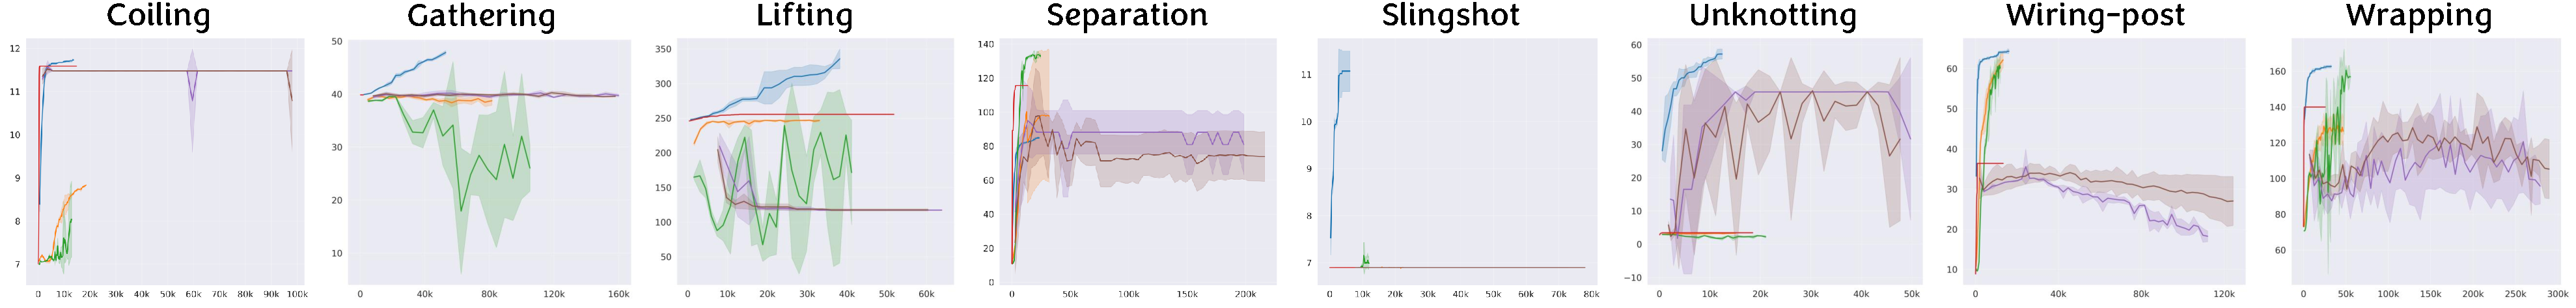
\includegraphics[width=\linewidth]{figs/curves_b_v2.pdf}
    \caption{\textbf{DLO-Lab tasks training curves.} We report episodic return as a function of wall-clock time in seconds for the 8 fixed-horizon tasks in our benchmark. Color correspondence: \textcolor[HTML]{ff7f0e}{\bf PPO}, \textcolor[HTML]{2ca02c}{\bf SAC}, \textcolor[HTML]{9467bd}{\bf SHAC}, \textcolor[HTML]{8c564b}{\bf SAPO}, \textcolor[HTML]{d62728}{\bf GD}, and \textcolor[HTML]{1f77b4}{\bf CMA-ES}. For trajectory optimization methods, we plot the prefix maximum.}
    \label{fig:curve_time}
\end{figure*}

\begin{table*}[t]
\centering
\scalebox{0.9}{
\setlength{\tabcolsep}{1.8mm}{
\begin{tabular}{l|cccccccc|c}
    \toprule
    \bf Tasks  & \bf Coiling & \bf Gathering & \bf Lifting & \bf Separation & \bf Slingshot & \bf Unknotting & \bf Wiring-post & \bf Wrapping & \bf Average \\
    \midrule
    \bf PPO      & 67\%  & 0\%  & 0\% & 100\%  & 0\%   & 0\% & 67\%  & 0\%  & 29.3\% \\
    \bf SAC      & 0\%  & 0\%  & 0\% & 100\%  & 33\%  & 0\% & 0\%  & 0\%  & 16.6\% \\
    \midrule
    \bf SHAC     & 93\%  & 0\% & 0\%  & 100\% & 0\% & 73\% & 0\%  & 0\%  & 33.3\% \\
    \bf SAPO     & 100\%  & 0\% & 0\%  & 100\% & 0\% & 80\% & 0\%  & 0\%  & 35.0\% \\
    \midrule
    \bf GD       & 100\% & 0\%   & 0\% & 100\% & 0\%  & 0\%  &  0\% & 0\% & 25.0\% \\
    \bf CMA-ES   & 100\% & 100\% & 87\% & 100\% & 93\%  & 93\%  & 93\%  & 27\% & 86.6\% \\
    \bottomrule
\end{tabular}
}}
\caption{\textbf{DLO-Lab tasks success rates.}}
    \label{tab:success_rate}
\vspace{-2mm}
\end{table*}

\begin{table}[ht!]
    \centering
    \scalebox{0.9}{
    \begin{tabular}{c|ccc}
    \toprule
    \bf Tasks & \bf Lifting & \bf Unknotting & \bf Wrapping \\
    \midrule
      \bf  Candidate Mode & \bf 335.59$\pm$14.21 & \bf 57.21$\pm$1.51 & \bf 162.68$\pm$0.86\\
      \bf  Coefficient Mode & 330.57$\pm$9.03 & 3.06$\pm$0.01 & 144.78$\pm$3.23\\
      \bf  Marker Mode & 330.57$\pm$9.03 & 3.06$\pm$0.01& 136.39$\pm$1.14\\
    \bottomrule
    \end{tabular}
    }
    \caption{\textbf{Comparison of different modes of the DLO agent for grasp proposal.} We use CMA-ES with the grasping points suggested by different modes and report the maximum episodic return. For other tasks, the suggested grasping points are generally the same.}
    \label{tab:agent_grasping_points}
\end{table}

\subsection{Training Curves based on Wall-Clock Time}
In~\Cref{fig:curve}, we present the training curves based on environment steps. Here, we plot these curves as a function of wall-clock time in seconds. The results are shown in~\Cref{fig:curve_time}.  It is evident that when informative gradients are available, the gradient-based trajectory optimization method (GD) can converge to a local minimum in just a few minutes. In contrast, the sample-based trajectory optimization method typically requires one to two hours to produce a satisfactory trajectory, although the final result often outperforms GD. In reinforcement learning (RL), the process typically takes several hours to tens of hours to develop a closed-loop policy.


\begin{figure*}[t]
    \centering
    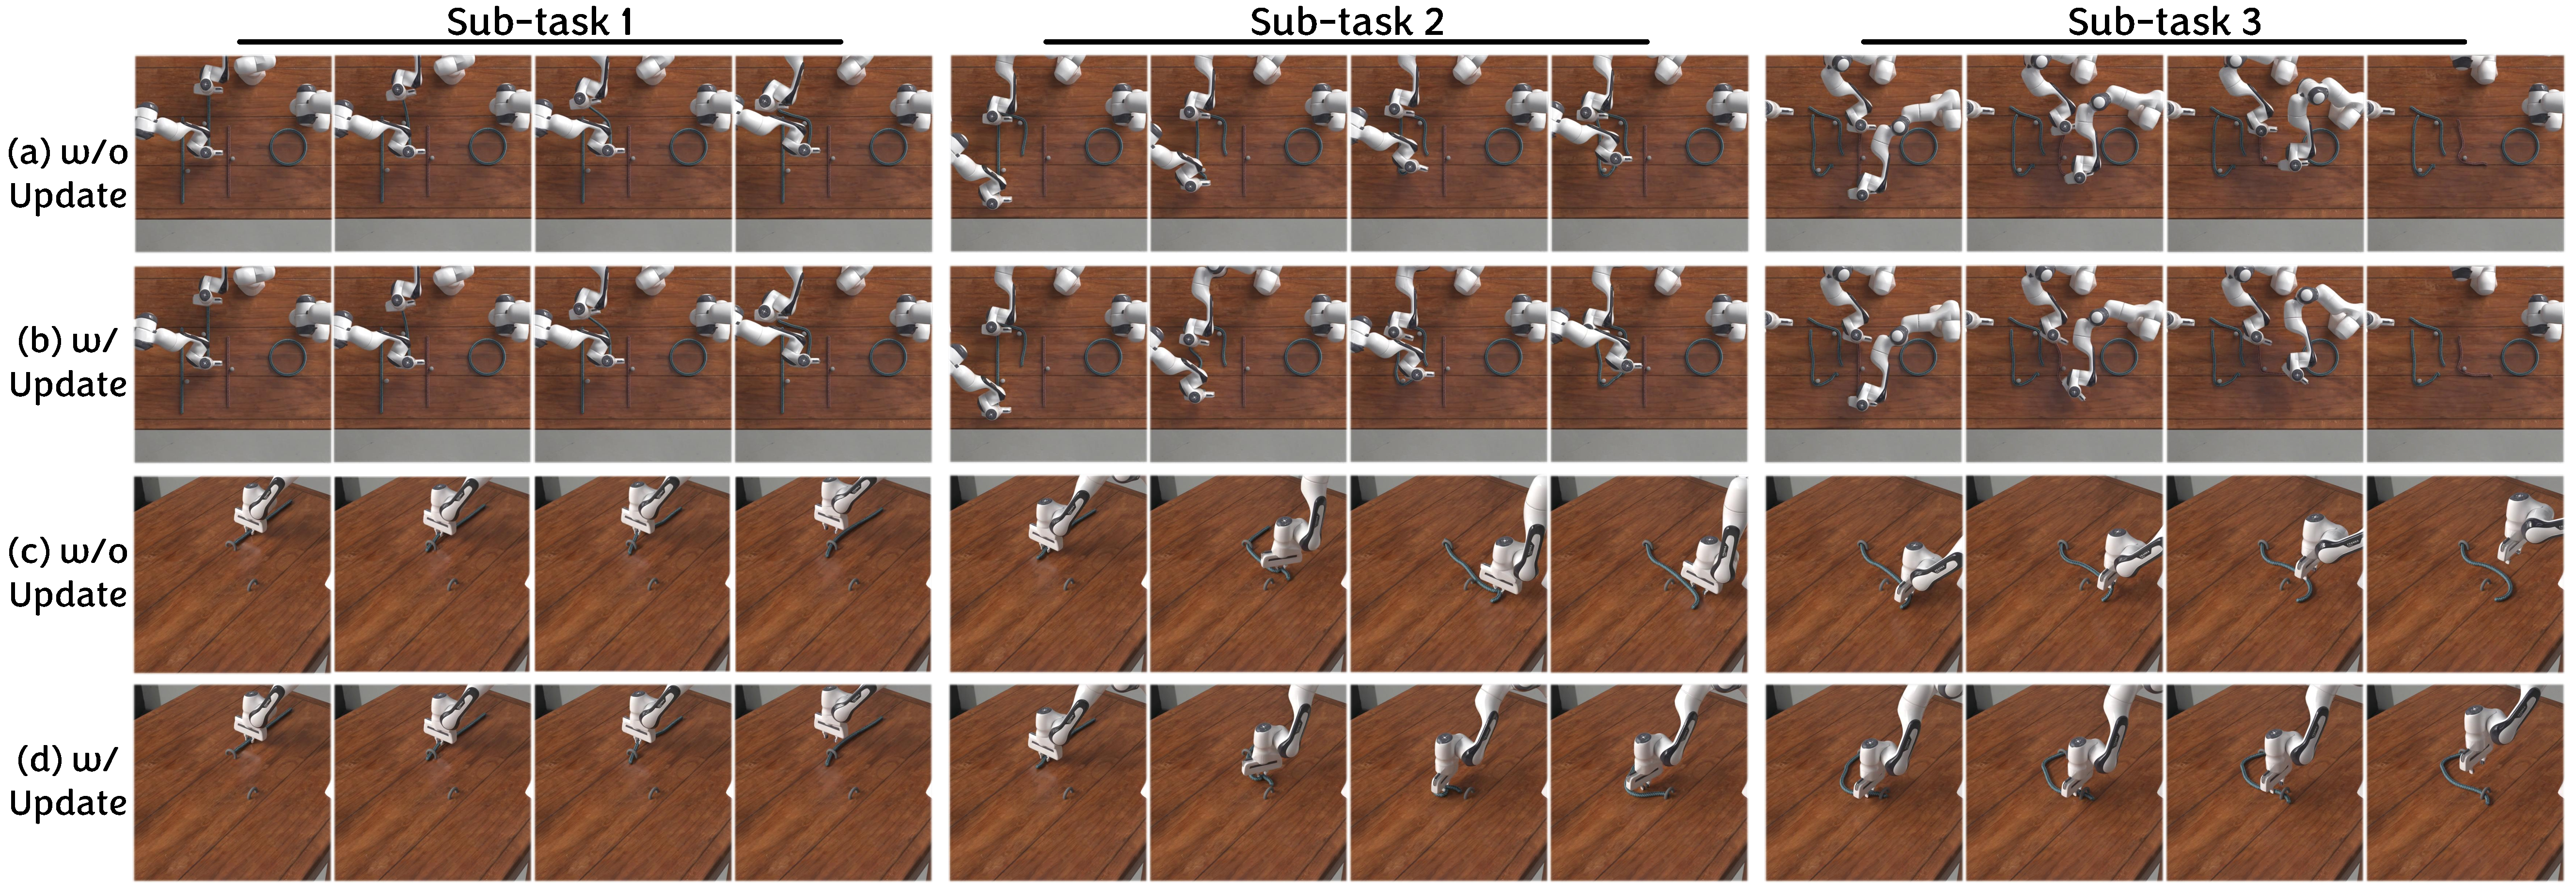
\includegraphics[width=1\linewidth]{figs/agent_task_decomposition_v2.pdf}
    \caption{\textbf{Analysis on the plan update strategy of the DLO agent for task decomposition.} We analyze the plan update strategy of the DLO agent in the (a-b) \textit{Letter Art} and (c-d) \textit{Wiring-ring} tasks. Without the plan update, the task decomposition plan is created at the start and remains fixed throughout the task. When the plan is updated after completing each sub-task, the agent can adjust sub-task rewards and dynamically re-plan sub-tasks, helping achieve the overall goal more effectively.}
    \label{fig:agent_task_decomposition_comparison}
\end{figure*}

\subsection{Success Rates}
\label{sec:success_rate}
To provide an intuitive understanding of the performance of different methods on our benchmark tasks, we assess their success rates in~\Cref{tab:success_rate}. Specifically, for RL algorithms, \ie, PPO, SAC, SHAC, and SAPO, we evaluate 15 trajectories for each algorithm across each task. In the case of GD, which is deterministic, we assess the final optimized trajectory for each task. For CMA-ES, we select the top 15 trajectories based on the returns from the best checkpoint. We determine the success of a trajectory by checking whether the agent achieves its goal at the end of the rendered videos.

\subsection{Comparison on Grasp Proposal}
\label{sec:comparison_grasp_proposal}
We quantitatively evaluate the efficacy of the three grasp proposal modes, \ie, \textit{Candidate}, \textit{Coefficient}, and \textit{Marker}, in \Cref{tab:agent_grasping_points}. To ensure fair comparison, the raw outputs from the \textit{Coefficient} and \textit{Marker} modes are post-processed by projecting the predicted locations onto the nearest DLO vertices to obtain valid 3D grasping coordinates. As evidenced by the results, \textit{Candidate} mode consistently outperforms the other strategies, achieving the highest episodic returns across all tested tasks. The performance gap is most pronounced in the \textit{Unknotting} task, where precision is paramount. We attribute this superiority to the formulation of the problem: \textit{Candidate} mode constrains the VLM's decision space to a discrete set of physically valid points, effectively transforming the challenge from a continuous spatial estimation task, which is prone to hallucination and projection errors, into a more robust selection task. Conversely, the \textit{Coefficient} and \textit{Marker} modes often suffer from minor spatial inaccuracies that, after snapping to the nearest vertex, result in suboptimal grasping policies.

\subsection{Analysis of Task Decomposition}
\label{sec:analysis_task_decomposition}
We evaluate our DLO agent for task decomposition in the \textit{Letter Art} and \textit{Wiring-ring} tasks with the sample-based trajectory optimization method, CMA-ES, in~\Cref{fig:agent_task_decomposition_comparison}. To validate the necessity of the dynamic plan update strategy, which closes the loop between high-level planning and low-level execution, we also compare the trajectories of the DLO agent with and without this feedback mechanism, \ie, rows (a)\&(c) vs. rows (b)\&(d). The results show that for tasks with spatially distinct and independent sub-goals, such as \textit{Letter Art} (a-b), the initial decomposition plan is sufficient and yields comparable performance. However, in sequential, precision-critical tasks like \textit{Wiring-ring} (c-d), this static approach is inadequate. Concretely, in~\Cref{fig:agent_task_decomposition_comparison}(c), the agent successfully threads the first ring but struggles to transition to the second ring. To explain, this difficulty arises from the rigidity of the pre-computed reward, which does not account for the rope's deformed state after the first interaction. In contrast, the dynamic plan update allows the agent to re-assess the intermediate state and develop highly specific reward functions tailored to the immediate manipulation phase. As observed in our experiments, after completing sub-task 1, the agent dynamically refines the objective for the second ring by dividing it into distinct phases. First, it generates a ``corridor'' reward (sub-task 2) to ensure precise radial alignment and a stable approach. This is followed by a ``tunneling'' reward (sub-task 3) that specifically incentivizes axial pushing while penalizing buckling. This adaptive re-planning maintains a dense, informative local optimization landscape, effectively correcting execution drift in long-horizon tasks.

\begin{figure*}[h!]
    \centering
    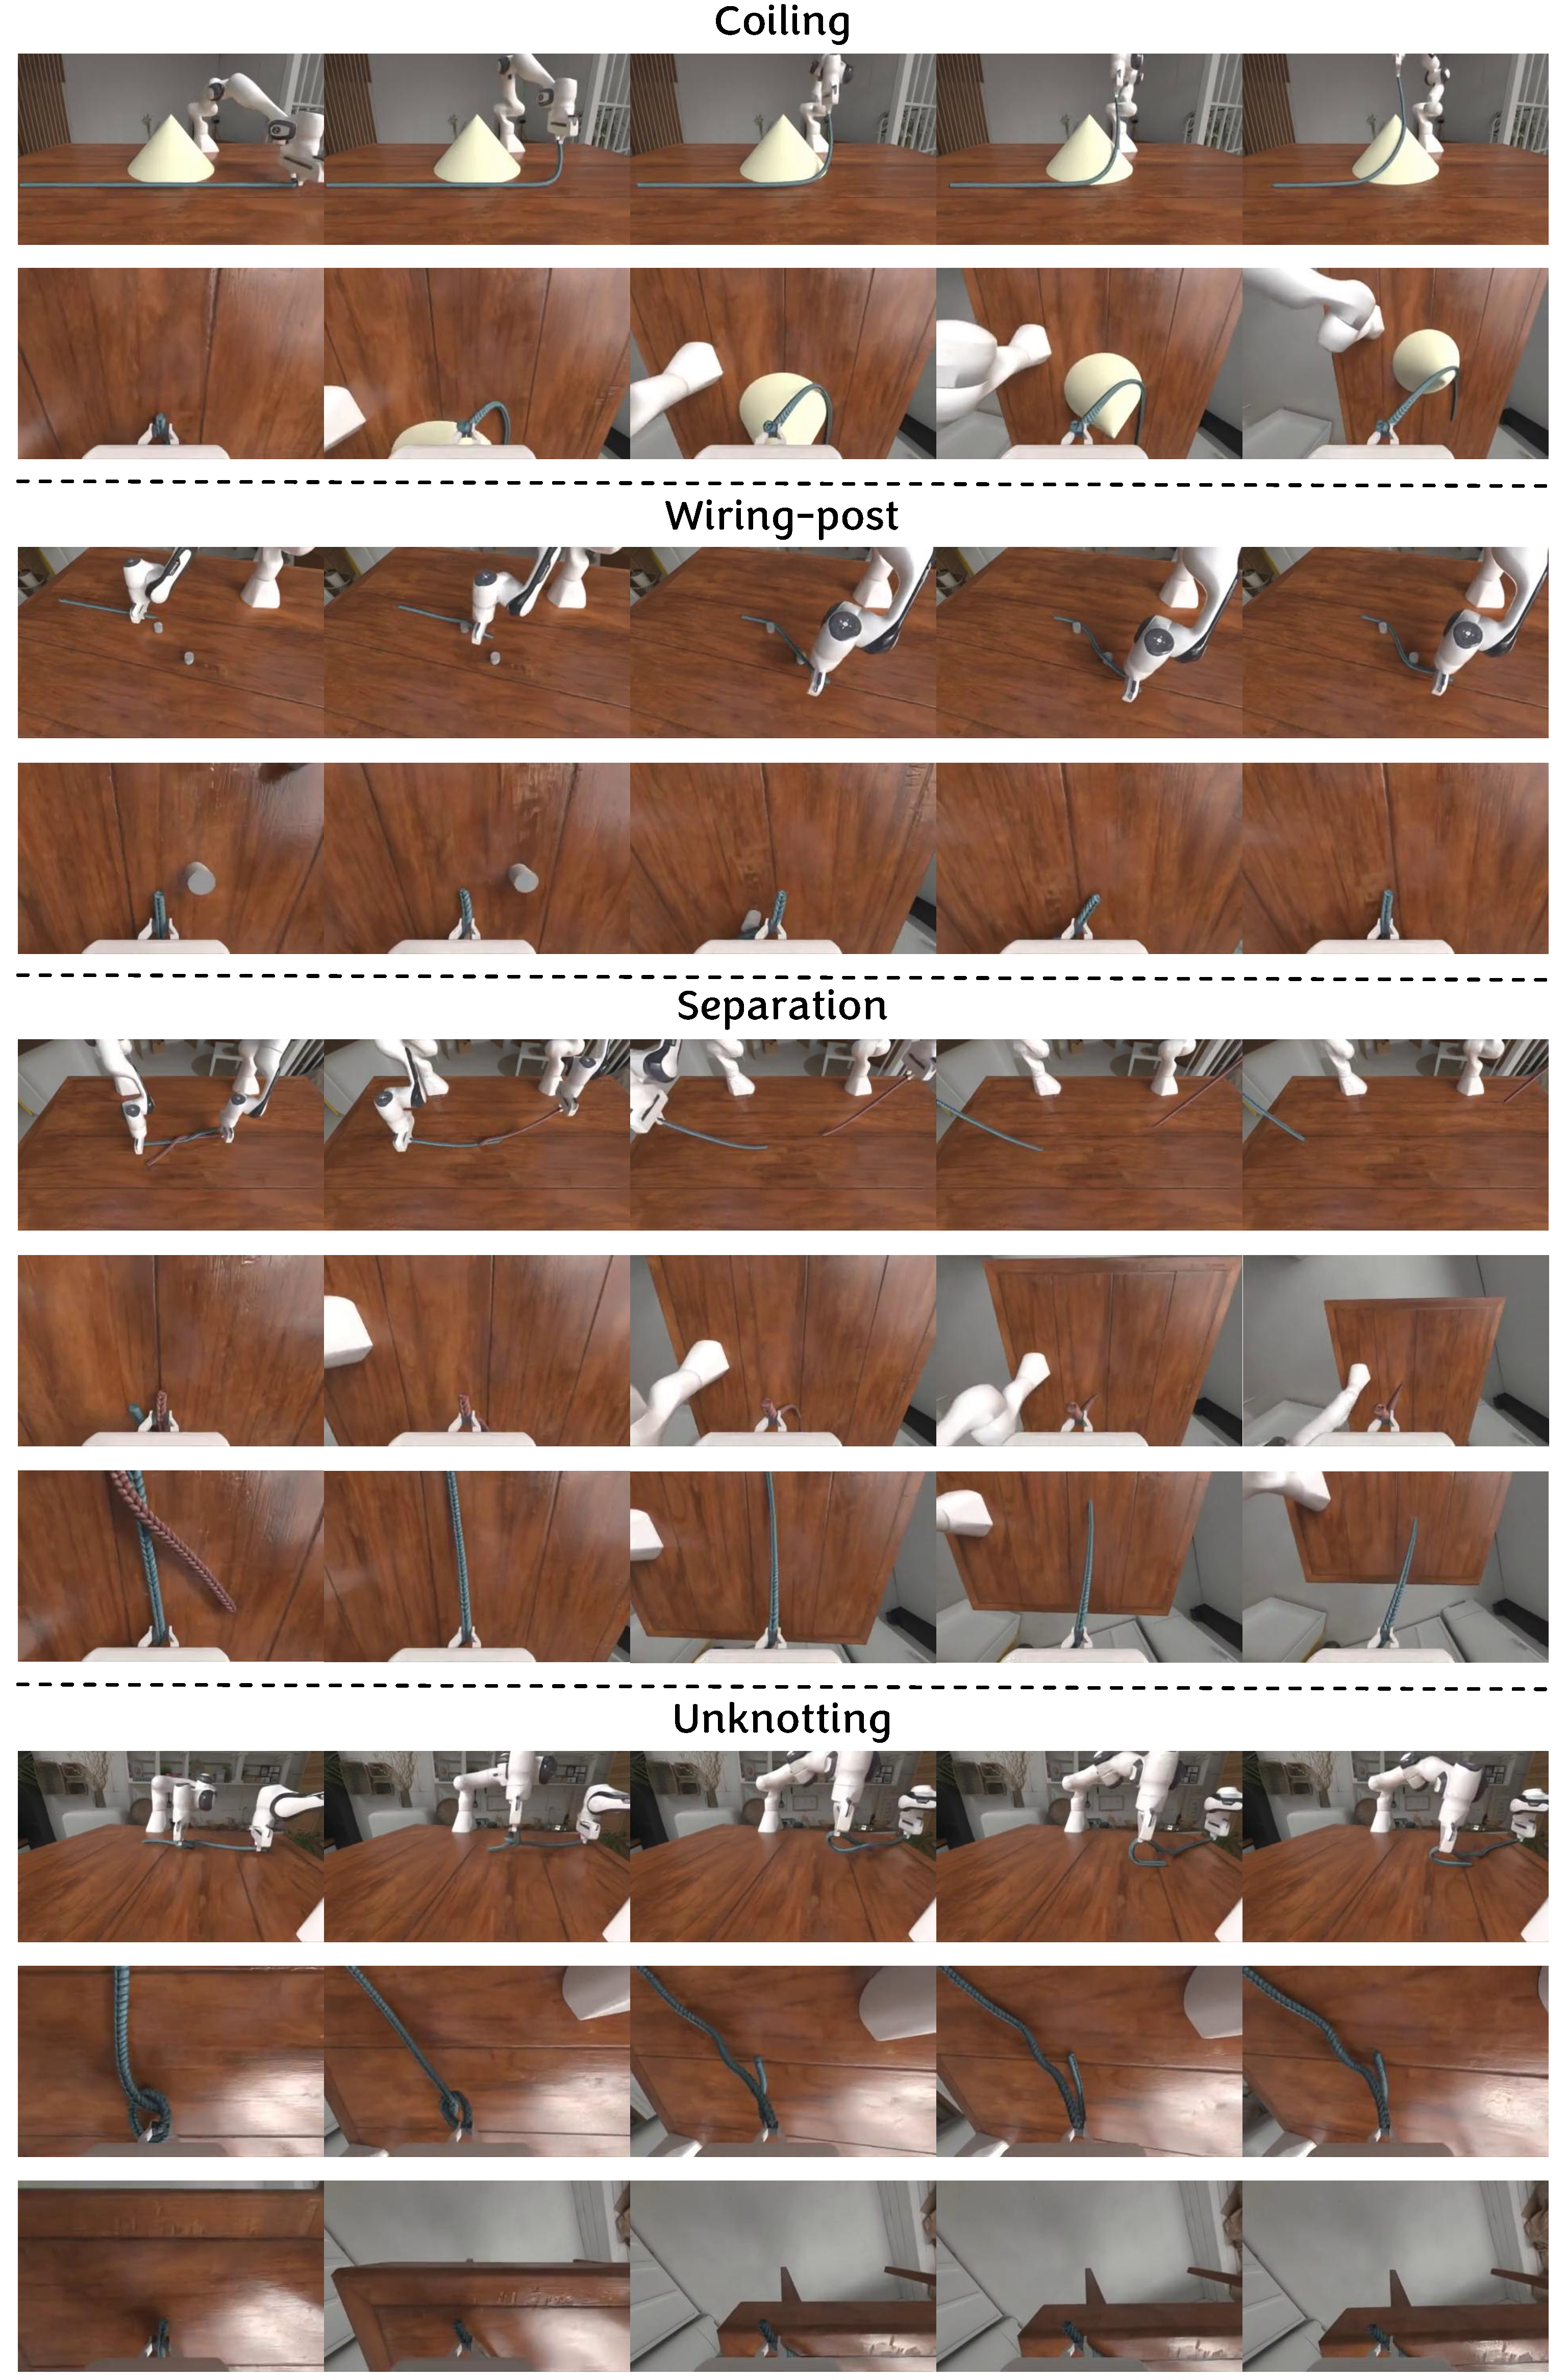
\includegraphics[width=.8\linewidth]{figs/data_sample_2.pdf}
    \caption{\textbf{Simulation demonstrations for VLA fine-tuning.} For each task, we display observations from the front camera (top row) and wrist camera(s) (subsequent rows).}
    \label{fig:data_sample}
\end{figure*}

\subsection{Data Generation and VLA Fine-tuning}
\label{sec:vla_finetuning}

Beyond single-task optimization, DLO-Lab can serve as a high-fidelity data engine for training generalizable visuomotor policies. We demonstrate this by collecting simulation demonstrations and fine-tuning a Vision-Language-Action (VLA) model, then evaluating it zero-shot as a single multi-task policy across four tasks from our benchmark simultaneously.

\paragraph{Data Collection}
Using the trained policies in DLO-Lab, we generate 200 successful demonstrations per task across four tasks---\textit{Coiling}, \textit{Separation}, \textit{Unknotting}, and \textit{Wiring-post}---yielding 800 demonstrations in total. Each episode records rich multi-view visual observations comprising one front-facing camera and one to two wrist cameras depending on the task (see~\Cref{fig:data_sample}), paired with the corresponding end-effector control actions in DLO-Lab's standardized controller format.

\paragraph{Model and Training}
We fine-tune SmolVLA~\cite{shukor2025smolvla}, an efficient open-source Vision-Language-Action model, on the combined 800-demonstration dataset with a batch size of 128 for 40K iterations. Crucially, a \emph{single} SmolVLA policy is trained jointly across all four tasks, whereas the RL baselines (PPO, SAC, SHAC, SAPO) each require a dedicated policy trained from scratch for each task.

\paragraph{Results}
We evaluate SmolVLA on 15 trajectories per task and report success rates in~\Cref{tab:vla_results}. The single multi-task SmolVLA policy achieves an average success rate of 60.0\%, competitive with per-task PPO (58.5\%) and substantially higher than per-task SAC (25.0\%). On \textit{Separation} and \textit{Unknotting}, SmolVLA matches the best RL methods, while \textit{Wiring-post} remains challenging due to the high precision required for tip insertion. These results demonstrate that DLO-Lab can function as a scalable synthetic data engine to bootstrap generalizable manipulation policies.

\begin{table}[h]
    \centering
    \scalebox{0.9}{
    \setlength{\tabcolsep}{1.5mm}{
    \begin{tabular}{l|cccc|c}
        \toprule
        \bf Method & \bf Coiling & \bf Separation & \bf Unknotting & \bf Wiring-post & \bf Average \\
        \midrule
        \bf PPO  & 67\% & 100\% & 0\%  & 67\% & 58.5\% \\
        \bf SAC  & 0\%  & 100\% & 0\%  & 0\%  & 25.0\% \\
        \bf SHAC & 93\% & 100\% & 73\% & 0\%  & 66.5\% \\
        \bf SAPO & 100\% & 100\% & 80\% & 0\% & 70.0\% \\
        \midrule
        \bf SmolVLA (multi-task) & 60\% & 100\% & 73\% & 7\% & 60.0\% \\
        \bottomrule
    \end{tabular}
    }}
    \caption{\textbf{Success rates for VLA fine-tuning.} RL baselines are per-task single-task policies. SmolVLA is evaluated as a single policy trained jointly on all four tasks. Each method is evaluated on 15 trajectories per task.}
    \label{tab:vla_results}
\end{table}

\section{Simulation Performance}
We benchmark the running time of our simulator in~\Cref{tab:running_time}. Note that the frame time in the simulation is 1e-3 seconds.

We further examine how well our simulator aligns with fundamental conservation laws, focusing specifically on the conservation of momentum during two distinct contact scenarios, as illustrated in~\Cref{fig:momentum}. The scenarios we simulate are ``Parallel Contact" and ``Inclined Contact." The corresponding plots on the right-hand side track the system's total momentum error over time. It is observed that the error magnitude ranges from approximately 1e-13 to 1e-14, indicating that our simulator effectively conserves momentum during these contact events.

\begin{table*}[t]
\centering
\scalebox{0.9}{
\setlength{\tabcolsep}{1.2mm}{
\begin{tabular}{c|c|cccccccc}
   \toprule
   \bf Tasks &\bf \#Envs & \bf Coiling & \bf Gathering & \bf Lifting & \bf Separation & \bf Slingshot & \bf Unknotting & \bf 
   Wiring-post & \bf Wrapping  \\
    \midrule
    \bf \multirow{4}{*}{Forward} & 1 & 90.85 & 32.31 & 50.03 & 87.20 & 90.08 & 80.70 & 90.82 & 83.71 \\
    & 10 & 873.73 & 175.79 & 418.94 & 819.08 & 829.03 & 725.73 & 883.78 & 752.17\\
    & 50 &4349.98  & 365.86 & 1736.94& 3372.44&3759.83 &3192.53 &4125.65 & 3327.49 \\
    & 100 & 8566.86 & 422.92 & 2625.83 & 4939.99  & 6120.69 & 5131.42 & 8531.82 & 5139.43 \\
    \midrule
    \bf \multirow{2}{*}{Forward \&} & 1 & 32.49 & 8.24 & 12.10 & 30.29 & 13.73 & 28.68 &31.13 & 31.17 \\
    & 10 & 344.25 & 52.00 & 53.37 & 267.77 & 106.72 & 211.16 & 282.10 & 186.84 \\
    \bf \multirow{2}{*}{Backward} & 50 &1465.67 & 184.28 & 153.30 & 1056.34 & 412.05 & 709.75 & 1382.38 & 670.37 \\
    & 100 & 3015.49 & 300.56 & 245.21 & 1655.18 &661.25 & 1134.70 & 2509.35 & 1048.17 \\
   \bottomrule
\end{tabular}
}}
\caption{\textbf{Running time on an NVIDIA L40s GPU.} We present the average frames per second (FPS) for each task.}
\label{tab:running_time}
\end{table*}


\begin{figure}
\centering
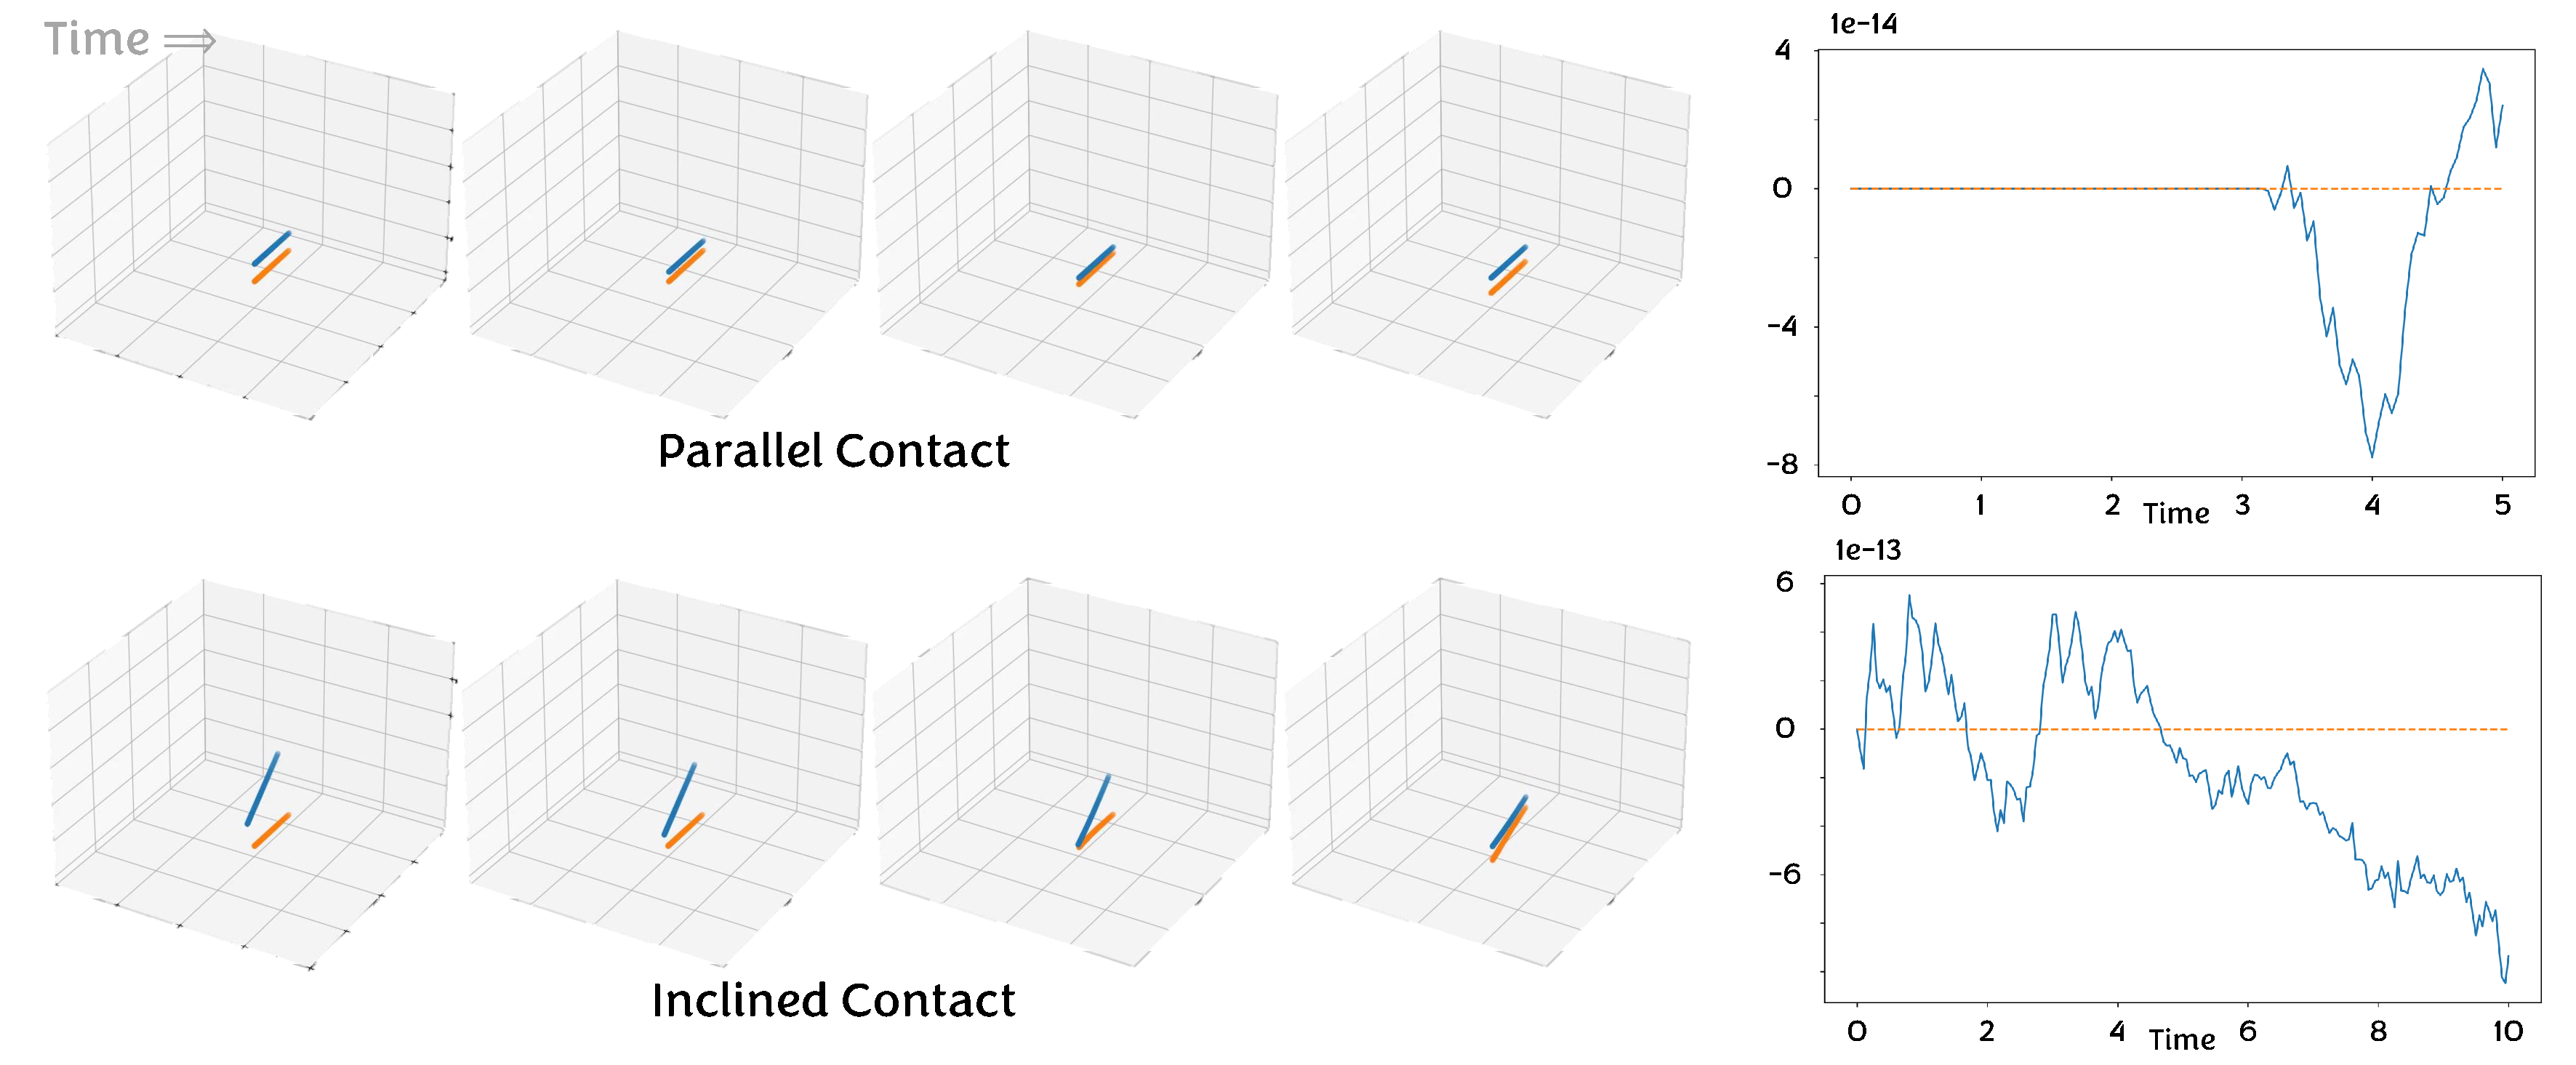
\includegraphics[width=1\linewidth]{figs/phys_check_v1.pdf}
    \caption{\textbf{Analysis of momentum conservation.} On the left, we display the contact cases we considered. On the right, we plot the system's total momentum error over time. Our simulator conserves momentum with very low errors during contact events.}
    \label{fig:momentum}
\end{figure}


\section{Real-World Relevance of Benchmark Tasks}
\label{sec:real_world_mapping}

In~\Cref{sec:manipulation_tasks}, we detail the DLO-Lab benchmark, designed to capture the diverse spectrum of real-world DLO manipulation challenges. Unlike prior works that often rely on abstract toy problems, we selected tasks that map directly to fundamental manipulation primitives essential in industrial manufacturing, logistics, and surgery. We explicitly connect our simulation scenarios to the following five core skills:
\begin{enumerate}[align=right,itemindent=0em,labelsep=2pt,labelwidth=1em,leftmargin=*,itemsep=0em] 
    \item \textbf{Cable Routing \& Threading}. Essential for industrial harnessing and surgical suturing, tasks like \textbf{Wiring-post} and \textbf{Wiring-ring} require guiding DLO tips through constrained apertures and specific channels with high precision.
    \item \textbf{Topological Manipulation}. Critical for cable maintenance and logistics, \textbf{Unknotting} and \textbf{Separation} demand reasoning about global topology to resolve complex knots and disentangle cluttered structures.
    \item \textbf{Winding \& Binding}. Mirroring coil winding and packaging processes, \textbf{Coiling} and \textbf{Wrapping} necessitate precise tension management to ensure DLOs conform tightly to rigid geometries.
    \item \textbf{Precision Shape Control}. Representing applications like wire bending for circuitry or catheter shaping, \textbf{Letter Art} challenges agents to deform DLOs into strict target geometries rather than loose functional configurations.
    \item \textbf{DLO-Mediated Manipulation}. Simulating tool use in scenarios like harvesting or construction, \textbf{Gathering}, \textbf{Lifting}, and \textbf{Slingshot} leverage the DLO's tension and shape to actuate, constrain, or propel other objects.
\end{enumerate}
Collectively, these tasks provide a rigorous and comprehensive testbed, ensuring that policies trained within our simulator possess the robust, transferable skills necessary for complex real-world deployment.


\section{Detailed Prompts of the DLO Agent}
\label{sec:details_dlo_agent}

Here, we provide the prompts used in our experiments for the two functionalities of the DLO agent. We use the Gemini-3-Pro-Preview model in this work.

\subsection{Grasp Proposal}
\paragraph{Candidate Mode} Below is the prompt we use for the \textit{Candidate} mode for the grasp proposal. 
\begin{lstlisting}[style=markdownstyle]
You are an intelligent AI assistant for robotics, physical simulation, and deformable object manipulation. 
Follow the user's requirements carefully and make sure you understand them. 
Keep your answers short and to the point. 
Do not provide any information that is not required. 

You will suggest grasping points for solving a manipulation task involving deformable linear objects (DLO), ensuring they are both efficient and robust for the task.
Here is the task description and reward definition:
{task_description}
{reward_description}

The dot markers with integer numbers in the attached images indicate the candidate grasping points on the DLO.
For this task, there are **{n_robots}** robots.
Here we calculate the distance from each grasping point to the basement of each robot:
{distance_info}

Using the information provided and your understanding of deformable manipulation, please recommend grasping points for each robot involved in the task. 
Please note that the grasping points will **not** be changed during the manipulation, so they should be chosen carefully to ensure successful task completion.

Please provide your answer in the following JSON format:
```
{
    "grasping_point_for_robot_1": ...       # An integer,
    "grasping_point_for_robot_2": ...       # (Optional) If applicable, an integer,
    "reasoning_for_the_suggestion": ...     # Provide a brief reasoning for your suggestion.
}
```

The output should **only** contain the JSON dictionary.
\end{lstlisting}

\paragraph{Coefficient Mode} Below is the prompt we use for the \textit{Coefficient} mode for the grasp proposal.
\begin{lstlisting}[style=markdownstyle]
You are an intelligent AI assistant for robotics, physical simulation, and deformable object manipulation. 
Follow the user's requirements carefully and make sure you understand them. 
Keep your answers short and to the point. 
Do not provide any information that is not required. 

You will suggest grasping points for solving a manipulation task involving deformable linear objects (DLO), ensuring they are both efficient and robust for the task.
Here is the task description and reward definition:
{task_description}
{reward_description}

The start and the end markers in the attached images indicate the starting vertex and the ending vertex of the DLO, respectively.
For this task, there are **{n_robots}** robots.
Here we calculate the distance from start or end vertex to the basement of each robot:
{distance_info}

Using the information provided and your understanding of deformable manipulation, please recommend grasping points for each robot involved in the task. 
The grasping points should be reprsented as coefficients in [0, 1], where 0 corresponds to the starting vertex and 1 corresponds to the ending vertex of the DLO.
Please note that the grasping points will **not** be changed during the manipulation, so they should be chosen carefully to ensure successful task completion.

Please provide your answer in the following JSON format:
```
{
    "grasping_point_for_robot_1": ...       # A float in [0, 1],
    "grasping_point_for_robot_2": ...       # (Optional) If applicable, a float in [0, 1],
    "reasoning_for_the_suggestion": ...     # Provide a brief reasoning for your suggestion.
}
```

The output should **only** contain the JSON dictionary.
\end{lstlisting}

\paragraph{Marker Mode} Below is the prompt we use for the \textit{Marker} mode for the grasp proposal.
\begin{lstlisting}[style=markdownstyle]
You are an intelligent AI assistant for robotics, physical simulation, and deformable object manipulation. 
Follow the user's requirements carefully and make sure you understand them. 
Keep your answers short and to the point. 
Do not provide any information that is not required. 

You will suggest grasping points for solving a manipulation task involving deformable linear objects (DLO), ensuring they are both efficient and robust for the task.
Here is the task description and reward definition:
{task_description}
{reward_description}

The start and the end markers in the attached images indicate the starting vertex and the ending vertex of the DLO, respectively.
For this task, there are **{n_robots}** robots.
Here we calculate the distance from start or end vertex to the basement of each robot:
{distance_info}

Using the information provided and your understanding of deformable manipulation, please recommend grasping points for each robot involved in the task. 
You need to mark the grasping points on the DLO in the **first** image by providing the image coordinates (x, y) in pixels (using OpenCV coordinate system).
For reference, the start and end vertex in the image have the following coordinates:
{coordinates_info}
Please note that the grasping points will **not** be changed during the manipulation, so they should be chosen carefully to ensure successful task completion.

Please provide your answer in the following JSON format:
```
{
    "grasping_point_for_robot_1": ...       # A tuple (x, y) representing image coordinates in pixels of the **first** image,
    "grasping_point_for_robot_2": ...       # (Optional) If applicable, a tuple (x, y) representing image coordinates in pixels of the **first** image,
    "reasoning_for_the_suggestion": ...     # Provide a brief reasoning for your suggestion.
}
```

The output should **only** contain the JSON dictionary.
\end{lstlisting}

\subsection{Task Decomposition}
\paragraph{Initial Decomposition Plan} Here is the prompt we use for obtaining the initial decomposition plan.
\begin{lstlisting}[style=markdownstyle]
You are an intelligent AI assistant for robotics, physical simulation, and deformable object manipulation. 
Follow the user's requirements carefully and make sure you understand them. 
Keep your answers short and to the point. 
Do not provide any information that is not required. 

You will divide a manipulation task for deformable linear objects into the fewest possible subtasks, keeping the robot gripper's grasping point on the linear object unchanged in each subtask. 
That is, break down the task into subtasks when a switch in grasping points is required to complete it. 

Here is the overall task description:
{task_description}

Here is the code snippet for the task environment setup:
{task_environment}

Using the information provided above, and the attached rendered images of the scene, decompose the task into the fewest possible subtasks.
Your response should be a list of dictionaries in JSON format, where each dictionary contains:
- "subtask_id": An integer representing the subtask number (starting from 1).
- "subtask_description": A brief description of the subtask.
- "reward_function": A code snippet defining the reward function for the subtask using the provided environment setup.
- "reward_description": A brief description in natural language of the reward function.
- "horizon_length": An integer specifying the maximum number of action steps allowed to complete the subtask.

Finally, you should append a dictionary with one key-value pair describing the overall task completion criteria after the list of subtasks, i.e.,
- "overall_task_completion_criteria": A brief description in natural language of the criteria for successfully completing the overall task.

Ensure that the subtasks are sequential and collectively achieve the overall task goal.

Make sure to format your response as valid JSON. The output should **only** contain the JSON list of subtasks and the overall task completion criteria.
\end{lstlisting}

\paragraph{Plan Update} Here is the prompt we use for evaluation and plan update after completing the optimization of each sub-task.
\begin{lstlisting}[style=markdownstyle]
You are an intelligent AI assistant for robotics, physical simulation, and deformable object manipulation. 
Follow the user's requirements carefully and make sure you understand them. 
Keep your answers short and to the point. 
Do not provide any information that is not required. 

You are working on subtask {subtask_id} of a larger manipulation task for deformable linear objects. 
Here is the overall task description:
{task_description}

Here is the code snippet for the task environment setup:
{task_environment}

The original task decomposition plan for the whole task is as follows:
{previous_plan}

Given the current state of the environment, you should:
(1) first judge whether the overall task has been completed successfully after executing subtask {subtask_id};
(2) if the overall task is not yet completed, update subsequent subtasks in the previous plan as necessary to ensure successful completion of the overall task.

Specifically, here is the optimized trajectory from the robot's execution of subtask {subtask_id} (attached as rendered videos).
Here is the final state of the environment after executing subtask {subtask_id}:
{subtask_final_state}

Using the information above, you may update the subtasks following subtask {subtask_id} to account for any changes in the environment or object state resulting from the execution of subtask {subtask_id}.
Your response should be a list of dictionaries in JSON format,
(1) if the overall task has been completed successfully, return a list with a single dictionary:
- "reasoning_for_completion": A brief explanation in natural language of why the overall task is considered completed successfully after executing subtask {subtask_id};
(2) otherwise, return the updated plan, i.e., the list of dictionaries where each dictionary contains:
- "subtask_id": An integer representing the subtask number (starting from {subtask_id + 1}, representing the next and subsequent subtasks).
- "subtask_description": A brief description of the subtask.
- "reward_function": A code snippet defining the reward function for the subtask using the provided environment setup.
- "reward_description": A brief description in natural language of the reward function.
- "horizon_length": An integer specifying the maximum number of action steps allowed to complete the subtask.
Ensure that the subtasks are sequential and collectively achieve the overall task goal.

Make sure to format your response as valid JSON. The output should **only** contain the JSON list of subtasks and the overall task completion criteria.
\end{lstlisting}

\section{Future Directions}
While DLO-Lab establishes a comprehensive platform for learning deformable manipulation, our benchmark results indicate that no single optimization strategy currently suffices for all tasks. Gradient-based methods are efficient but tend to struggle with non-smooth landscapes, whereas sampling-based approaches provide robustness but come with higher computational costs. A promising direction for future research is the development of hybrid optimization algorithms that combine the strengths of these two methods. For example, integrating zeroth-order sampling with first-order analytic gradients could effectively balance the bias-variance trade-offs often encountered in differentiable physics, as suggested by \citep{suh2022differentiable}. Additionally, we believe an interesting area for exploration is enhancing the DLO agent's capabilities to overcome the specific limitations of gradient-based trajectory optimization methods in indirect manipulation tasks. By leveraging the agent to plan initialization trajectories that create stable contact, we can address challenges in sparse-reward scenarios, such as tool use. This approach will allow the optimizer to take over once effective gradient flows are established. Finally, while we have demonstrated zero-shot sim-to-real transfer in both open-loop and closed-loop settings, improving the robustness and coverage of this pipeline remains an open challenge. In particular, more reliable real-time DLO state estimation across diverse objects and environments, as well as scaling synthetic demonstration generation for broader visuomotor policy training, are promising avenues for future work.